% SN-LPA architecture flowchart (moved out of the paper). Compile: tectonic sn_lpa_architecture.tex
% Caption used in the paper: Architecture of the proposed pipeline. Orange boxes modify a step of TPOC-LPA, blue boxes are new steps, white boxes are unchanged (compare Fig.~\ref{fig:base}).
\documentclass[border=6pt]{standalone}
\usepackage{amsmath,amssymb}
\usepackage{tikz}
\usetikzlibrary{shapes.geometric,shapes.misc,arrows.meta,positioning,fit,backgrounds,calc}
\tikzset{
  term/.style={rounded rectangle, draw, thick, font=\scriptsize, minimum height=5mm, minimum width=12mm, fill=gray!12},
  io/.style={trapezium, trapezium left angle=72, trapezium right angle=108, draw, thick, font=\scriptsize, align=center, minimum height=6.5mm, fill=gray!8},
  proc/.style={rectangle, draw, thick, font=\scriptsize, align=center, minimum height=7mm, inner sep=2.5pt},
  dec/.style={diamond, aspect=2.4, draw, thick, font=\scriptsize, align=center, inner sep=1.5pt},
  newp/.style={proc, fill=blue!14},
  modp/.style={proc, fill=orange!28},
  arr/.style={-{Stealth[length=1.8mm,width=1.5mm]}, thick},
  lab/.style={font=\scriptsize\itshape, inner sep=1pt}
}
\begin{document}
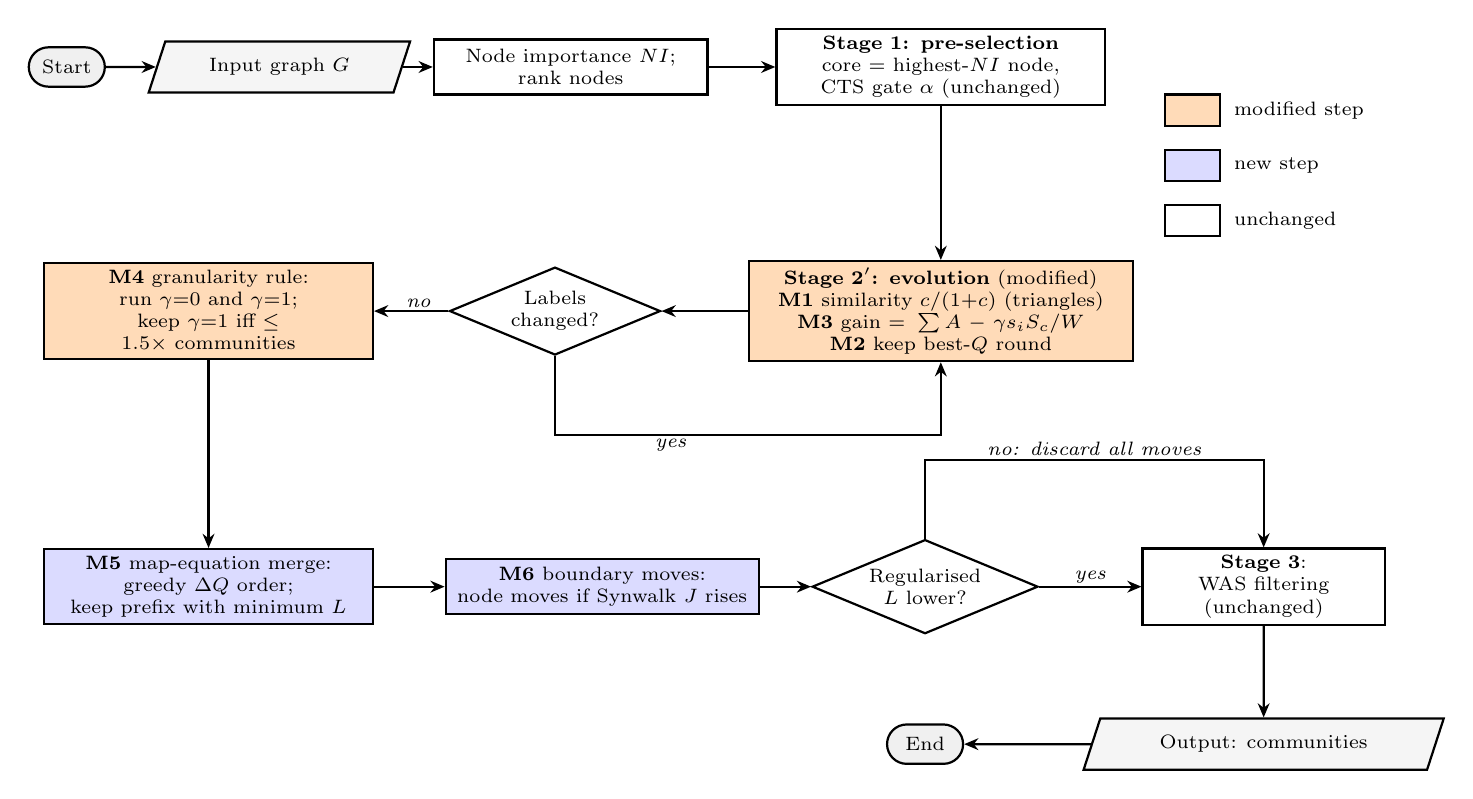
\begin{tikzpicture}[x=1cm,y=1cm]
\node[term] (s) at (0.8,0) {Start};
\node[io] (in) at (3.5,0) {Input graph $G$};
\node[proc, text width=33mm] (ni) at (7.2,0) {Node importance $NI$;\\ rank nodes};
\node[proc, text width=40mm] (s1) at (11.9,0) {\textbf{Stage 1: pre-selection}\\ core = highest-$NI$ node,\\ CTS gate $\alpha$ (unchanged)};
\node[modp, text width=47mm] (s2) at (11.9,-3.1) {\textbf{Stage 2$'$: evolution} (modified)\\ \textbf{M1} similarity $c/(1{+}c)$ (triangles)\\ \textbf{M3} gain $=\sum A-\gamma s_iS_c/W$\\ \textbf{M2} keep best-$Q$ round};
\node[dec] (d2) at (7.0,-3.1) {Labels\\changed?};
\node[modp, text width=40mm] (m4) at (2.6,-3.1) {\textbf{M4} granularity rule:\\ run $\gamma{=}0$ and $\gamma{=}1$;\\ keep $\gamma{=}1$ iff $\le1.5\times$ communities};
\node[newp, text width=40mm] (m5) at (2.6,-6.6) {\textbf{M5} map-equation merge:\\ greedy $\Delta Q$ order;\\ keep prefix with minimum $L$};
\node[newp, text width=38mm] (m6) at (7.6,-6.6) {\textbf{M6} boundary moves:\\ node moves if Synwalk $J$ rises};
\node[dec] (g) at (11.7,-6.6) {Regularised\\$L$ lower?};
\node[proc, text width=29mm] (s3) at (16.0,-6.6) {\textbf{Stage 3}: WAS filtering\\ (unchanged)};
\node[io] (out) at (16.0,-8.6) {Output: communities};
\node[term] (e) at (11.7,-8.6) {End};
\draw[arr] (s)--(in); \draw[arr] (in)--(ni); \draw[arr] (ni)--(s1);
\draw[arr] (s1)--(s2);
\draw[arr] (s2)--(d2);
\draw[arr] (d2.south) -- ++(0,-1.0) -| (s2.south) node[lab, pos=.15, below]{yes};
\draw[arr] (d2)--(m4) node[lab, pos=.4, above]{no};
\draw[arr] (m4)--(m5);
\draw[arr] (m5)--(m6);
\draw[arr] (m6)--(g);
\draw[arr] (g)--(s3) node[lab, pos=.5, above]{yes};
\draw[arr] (g.north) -- ++(0,1.0) -| (s3.north) node[lab, pos=.25, above]{no: discard all moves};
\draw[arr] (s3)--(out); \draw[arr] (out)--(e);
\node[proc, fill=orange!28, minimum width=7mm, minimum height=4mm] at (15.1,-0.55) (l1) {};
\node[font=\scriptsize, anchor=west] at (15.5,-0.55) {modified step};
\node[proc, fill=blue!14, minimum width=7mm, minimum height=4mm] at (15.1,-1.25) (l2) {};
\node[font=\scriptsize, anchor=west] at (15.5,-1.25) {new step};
\node[proc, minimum width=7mm, minimum height=4mm] at (15.1,-1.95) (l3) {};
\node[font=\scriptsize, anchor=west] at (15.5,-1.95) {unchanged};
\end{tikzpicture}
\end{document}
